\section{Auswertung}
\subsection{Streuprobe}
Bevor man Röntgenfluoreszenzmessungen an tatsächlichen Proben vornimmt, ist es von großem Interesse mehr über den Anregungsstrahl und das produzierte Spektrum zu erfahren. Hierfür wurde eine ASB Streuprobe benutzt, um das Anregungsspektrum weitgehend unverändert zu untersuchen. Dabei wird davon ausgegangen das keine nennenswerten Absorptionen des Spektrums in der Probe oder Fluoreszenz in der Probe bei der Streuung auftreten. Das Spektrum ist jedoch nicht vollständig unverändert, es wird zum Beispiel Compton-Streuung beobachtet. Welche durch Wechselwirkung eines Photons mit einem Elektron Energie an diesen verliert, so dass die Wellenlänge des Photons dadurch verlängert wird \\
Zunächst wurde das Spektrum ohne Filter betrachtet, hierbei ist aufgefallen, dass ein relativ rauscharmes und kontinuierliches Spektrum bei einem „Total Counts“ Wert von ca. 2000 cps bei einer Messzeit von min 50s erreicht wird. Das Hintergrund Rauchen des Spektrums kann durch die Messzeit gut kontrolliert werden da es bei einer längeren Messzeit das Rauschen besseren numerisch rausrechenbar ist. Bei einer geringen Anregung Energie oder beim Einsatz von Absorptionsfilter muss allerdings die Messzeit erhöht werden um das Rauschen adäquat zu minimieren. Bei einer Messung mit einer Hochspannung von 50 keV und ohne den Einsatz eines Absorptionsfilters sind beispielweise relative rauscharme Speckten bei ca. 50 s Messzeit messbar. \\
Nach Verstellung der Hochspannung der Röntgenröhre (10 – 50 keV) und den einsetzen von Absorptionfilter am anregungsstrahl (Al 100-1000 µm, Ni 10 µm und My 100 µm) musste immer die Messzeit so angepasst werden das ein Rauscharmes Spektrum Messbar wurde. In der Tabelle \ref{fig:Filter} sind einige Beispiele gelistet mit dem ein zufriedenstellendes Spektrum erzeugt wurde.\\
\begin{figure}[h]
 \centering
 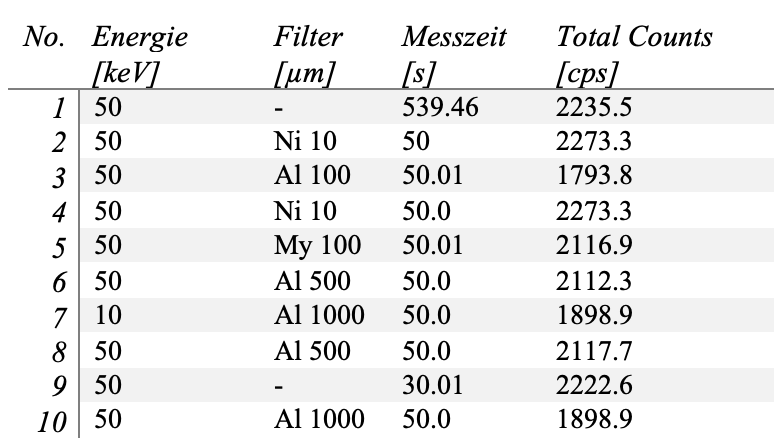
\includegraphics[width=0.7\textwidth]{Filter.png}
 \caption[Filter Tabelle]{Tabelle aller verwendeten Tabelle aller verwandten Filter Einstellungen bei Streuprobe}
 \label{fig:Filter}
\end{figure}
Auf der Abbildung \ref{fig:Filter} ist das Streuspektrum dargestellt hier kann man sehr gut die zu erwartende kontinuierliche kurve der Röntgenröhre erkennen, diese wird durch die Bremsstrahlung der Elektronen an der Anode Verursacht. Bei dem Beispiel in Abbildung \ref{fig:example} gezeigtem Spektrum ist die komplette Bandbreite bis hin zum 50 keV zu sehen, eine höhere Energie ist nicht zu erwarten da die gesamte Energie eines Elektrons mit maximal 50 keV an ein Photon abgegeben wird. Die Energieverteilungskurve hat hierbei ein Maximum bei ca. 10 keV.
Durch das Streuspektrum können einige weite Eigenschaften des Messinstruments festgestellt werden. Eine Reihe dieser Peaks können durch Rhodium erklärt werden. Zunächst sind die Rh K$\alpha_1 $ bei 20,33 keV, die Rh L $\alpha_1$ bei 2,70 keV und die Rh L $\beta_1$ Floreszenz Peaks zu erkennen, dass vorhanden sein dieser Peaks last darauf schließen das die Anode der Röntgenröhre aus Rhodium gefertigt ist. Ein breiterer Peak bei der Energie von 18,9 keV lässt sich auf die Compton Streuung der Rh K$\alpha_1 $ Peak zurückführen. Der scharfe Peak bei der Energie von 21,2 keV ist hingegen durch die Rayleigh Streuung zu erklären.\\
Außerdem kann ein Argon K$\alpha$ Peak identifiziert werden, dies ist durch die Luft im Röntgenstrahl erklärbar, da der Versuchsaufbau nicht in einem Vakuum vorgenommen wird.\\
Die Verkleinerung der Hochspannung der Röntgenröhre hat den Effekt, dass das Streuspektrum modifiziert wird. Dabei wird das Spektrum nur bis zur Energie der Hochspannung erzeugt. Es ist im Vergleich zur maximal höchsten Spannung von 50kV abgeschnitten. Zusätzlich ist die Intensitätsverteilung der gesamten kurve im Vergleich kleiner\\
Durch den Einsatz von Absorptionsfilteren vor dem Anregungsstrahl kann das Spektrum zusätzlich modifiziert, hierbei sind zwei Effekte beobachtbar.
Zum einen wird die gesamte Zahl der gemessenen Photonen über dem gesamten Spektrum reduziert. Zum anderen werden je nach Filter Material gewisse Regionen im Spektrum geblockt. In dieser Region ist die Absorption des filtermaterial besonderes stark, dadurch können weniger Photonen in diesem Energiebereich an der Probe gestreut werden und dementsprechend gemessen werden. Eine Probe kann dennoch in diesem Bereich Fluoreszieren, wenn die anregungsbedingen des Anregungsstrahls dennoch ausreichen hierfür sind.\\
Mit Zuhilfenahme und Anpassung dieser Anregungsbedingungen, können bestimmte Regionen im Spektrum besonders hervorgehoben werden und präziser untersucht werden.\\


\begin{figure}%
    \centering
    \subfloat[\centering Kein Filter ]{{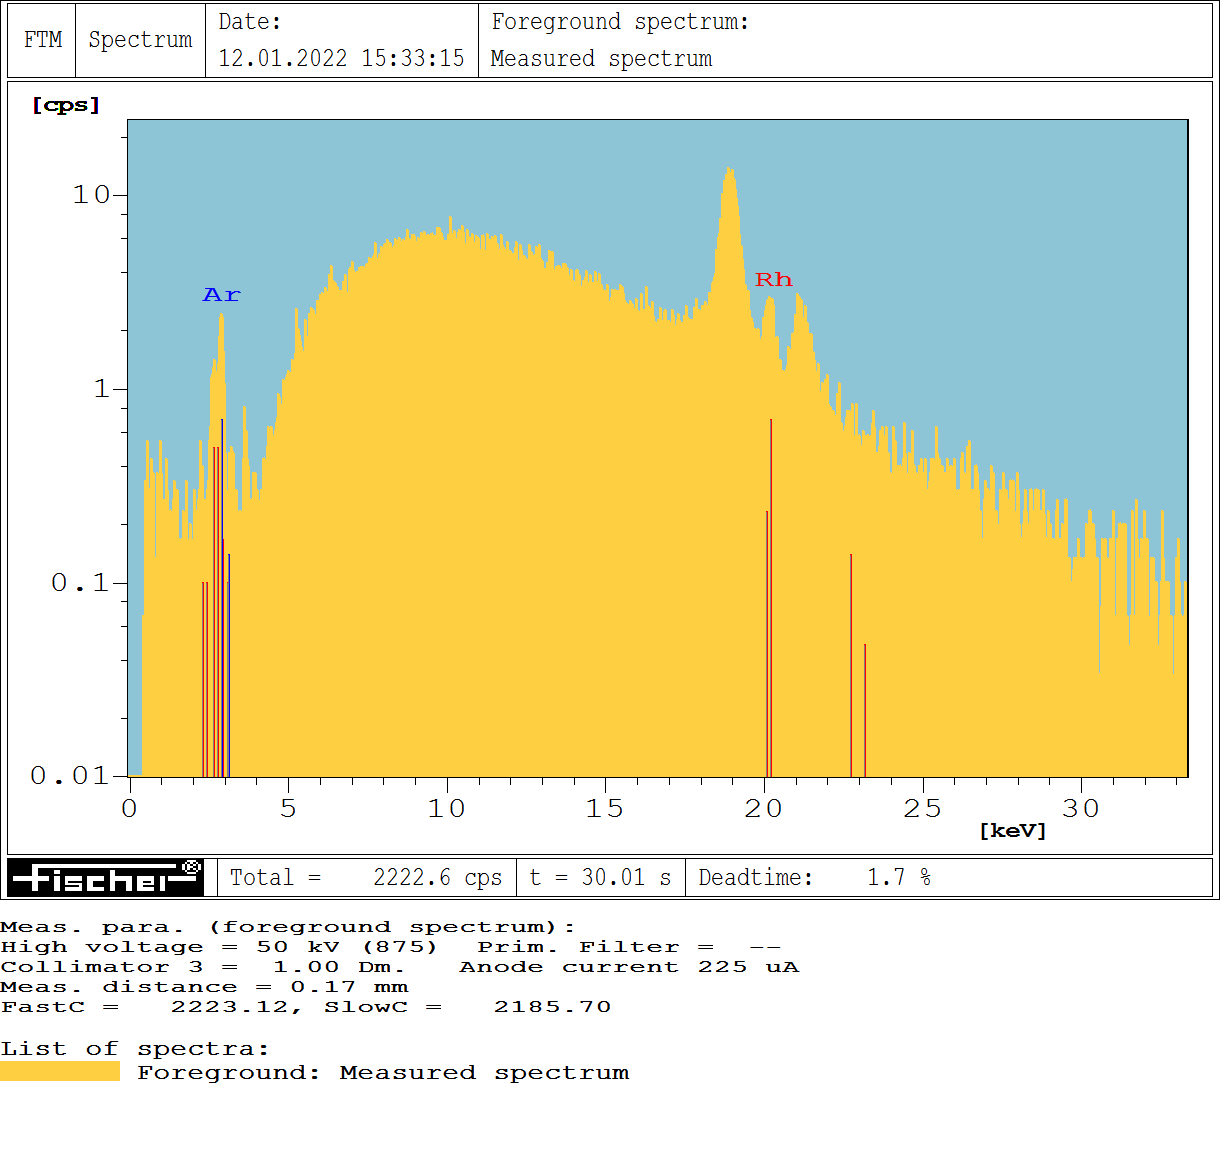
\includegraphics[width=7cm]{9_StreuSprectrumKeinFilter.png} }}%
    \qquad
    \subfloat[\centering 1000 µm Al Filter ]{{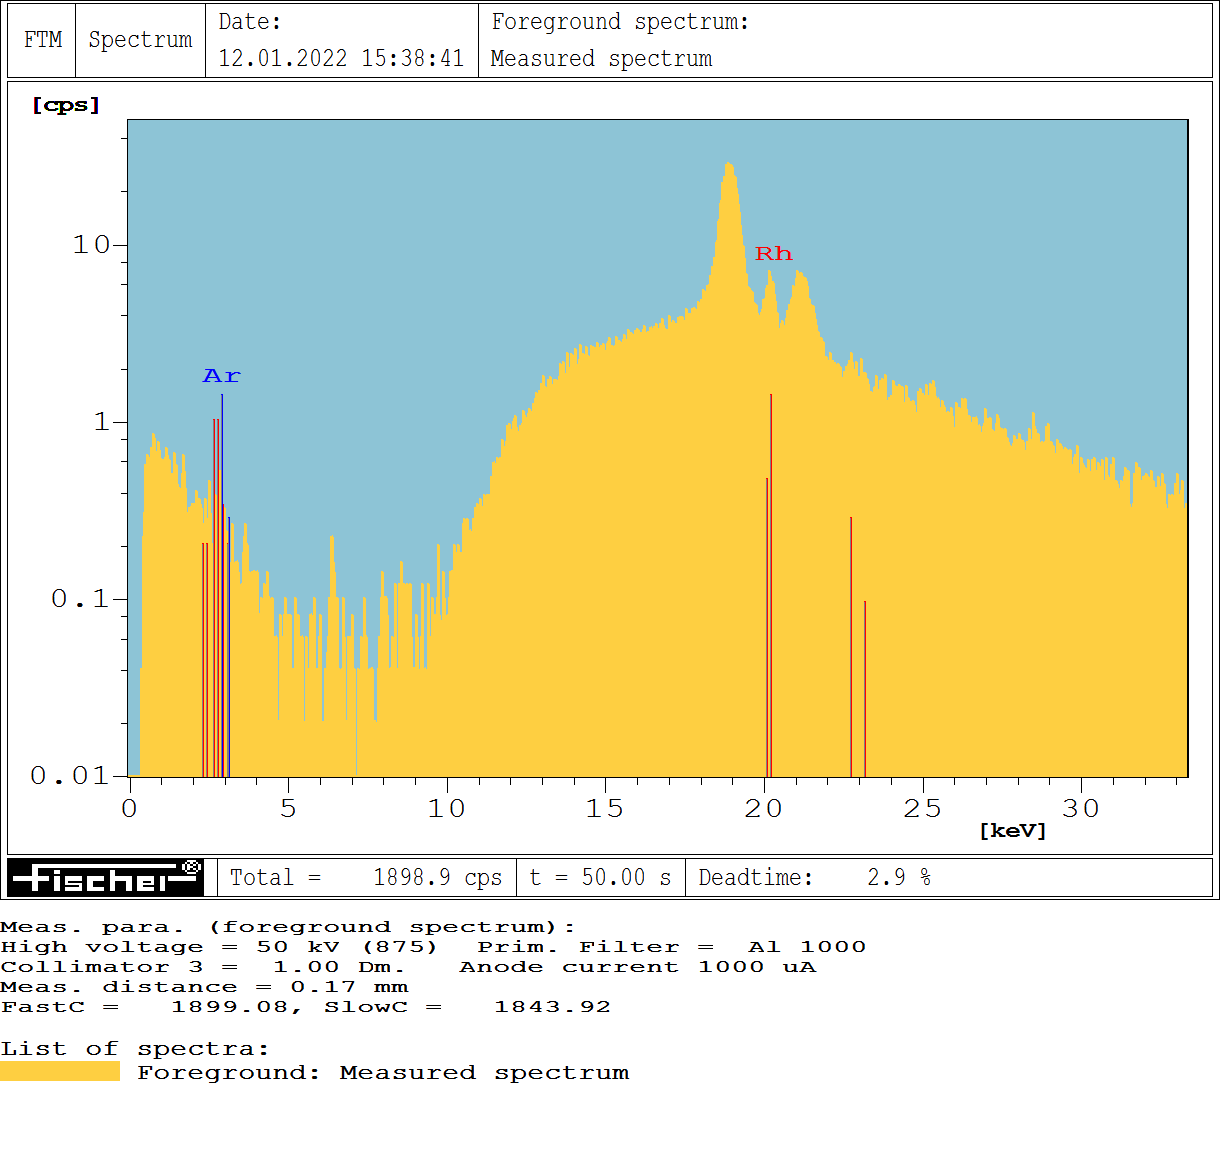
\includegraphics[width=7cm]{10_StreuStectrum1000Al.png} }}%
    \caption{Streuspektrum an ABS Probe bei 50kV Hochspannung, A) Spektrum ohne Filter, b) Spektrum mit 1000 µm Al Filter.}%
    \label{fig:example}%
\end{figure}


\subsection{Stahlprobe}
Um eine Stahlprobe auf ihre Zusammensetzung zu untersuchen, wurde sie zunächst bei einer Hochspannung von 50 kV und ohne Filter beleuchtet. Hierbei konnte sich ein erster Eindruck über das gesamte Spektrum gemacht werden und markante Peaks identifiziert werden. Dabei wurden die Ar und Rh wie bei der Streuprobe identifiziert.\\
Auch die sehr markanten Fe Peaks konnten identifiziert werden, die Peaks werden im Spektrum jedoch zwei Mal abgebildet. Zum ersten Mal sind es die eigentlichen Fe Peaks, beim zweiten Mal sind es die gleichen Peaks mit der doppelter Energie. Dies wird durch die Doppelmessung in Siliziumdriftdetektor verursacht, bei dem durch die starke Intensität dieser Peaks gleichzeitig zwei Photonen zur selben Zeit im Detektor gemessen wird. Die Energie der beiden Photonen wird dann zusammenaddiert. Die charakteristischen Mo, W, Cr und V Peaks sind bei dieser Anregungsbedingung auch leicht erkennbar.\\

\begin{figure}[h]
 \centering
 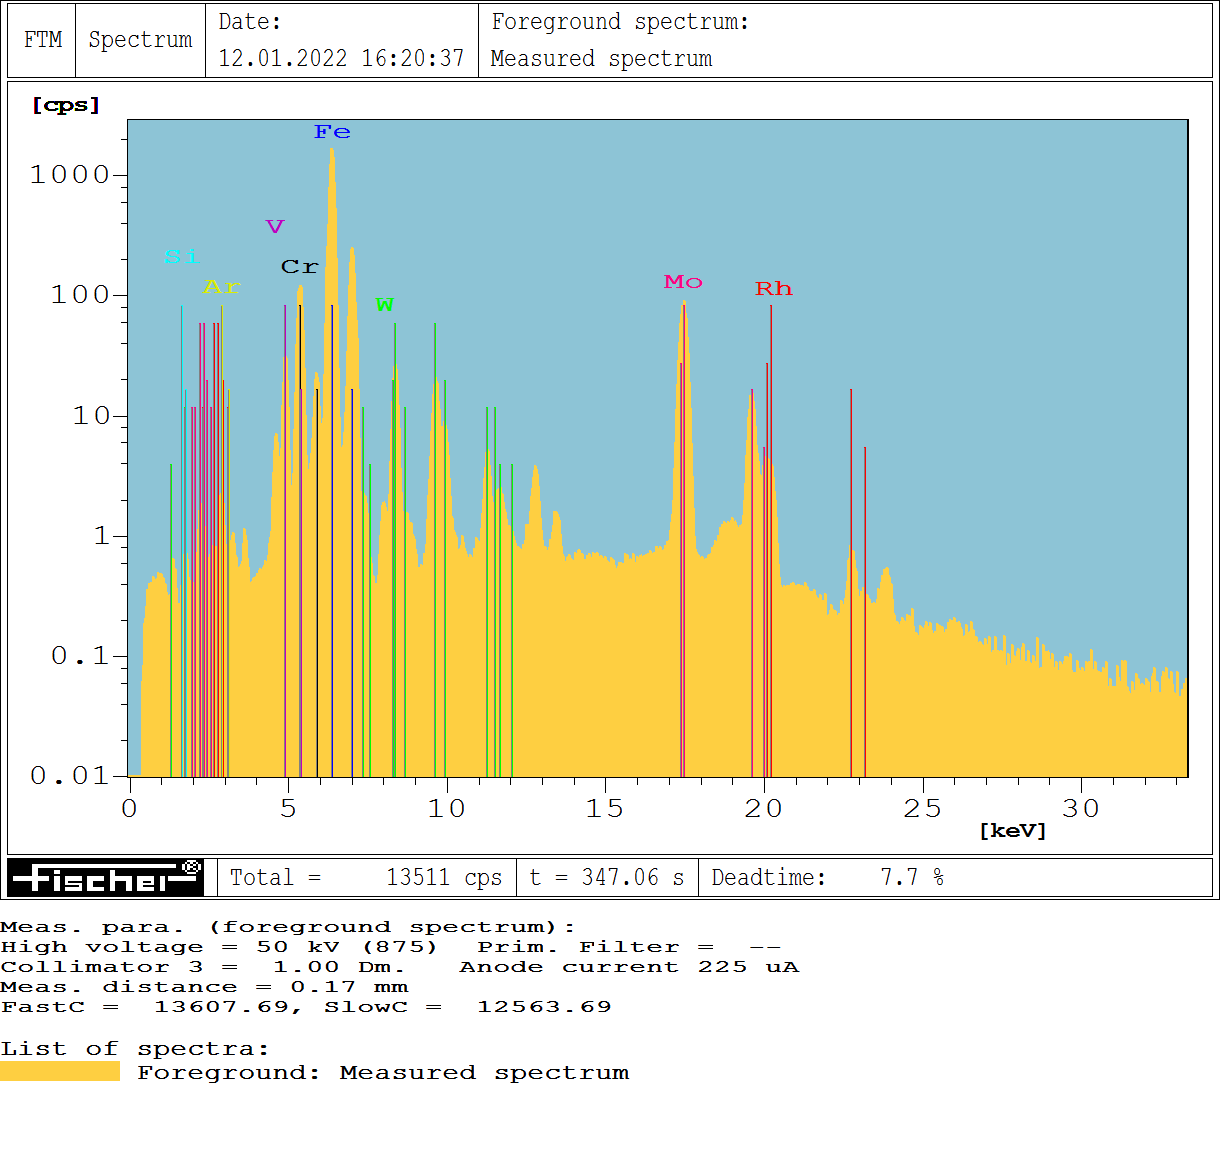
\includegraphics[width=0.5\textwidth]{Stahlprobe.png}
 \caption[Stahlprobe Sprktrum]{Spektrum der Stahlprobe bei 50keV und ohne filter.}
 \label{fig:Stahlprobe}
\end{figure}

Um die etwas kleinen Peaks zu identifizieren, wurde das „residual“ Spektrum in den interessanten Regionen genauer angeschaut.  Das Residual Spektrum ist die Differenz zwischen der erwarteten Intensität eines Peaks mit dem tatsachliche gemessenen Wert. Wenn das residuale Spektrum sehr Große Peaks aufweist kann davon ausgegangen werden, dass nicht alle Elemente der Probe korrekt identifiziert wurden. Zusätzlich konnten damit die Peaks von Mn identifiziert werden. Die dabei gemessene prozentuale Zusammensetzung der Stahlprobe ist in der Tabelle \ref{fig:Konzentration} aufgelistet. Die genormte Zusammensetzung des Herstellers, eingeschlossen nicht identifizierter Elemente sind ebenfalls in dieser Tabelle aufgelistet.\\

\begin{figure}[h]
 \centering
 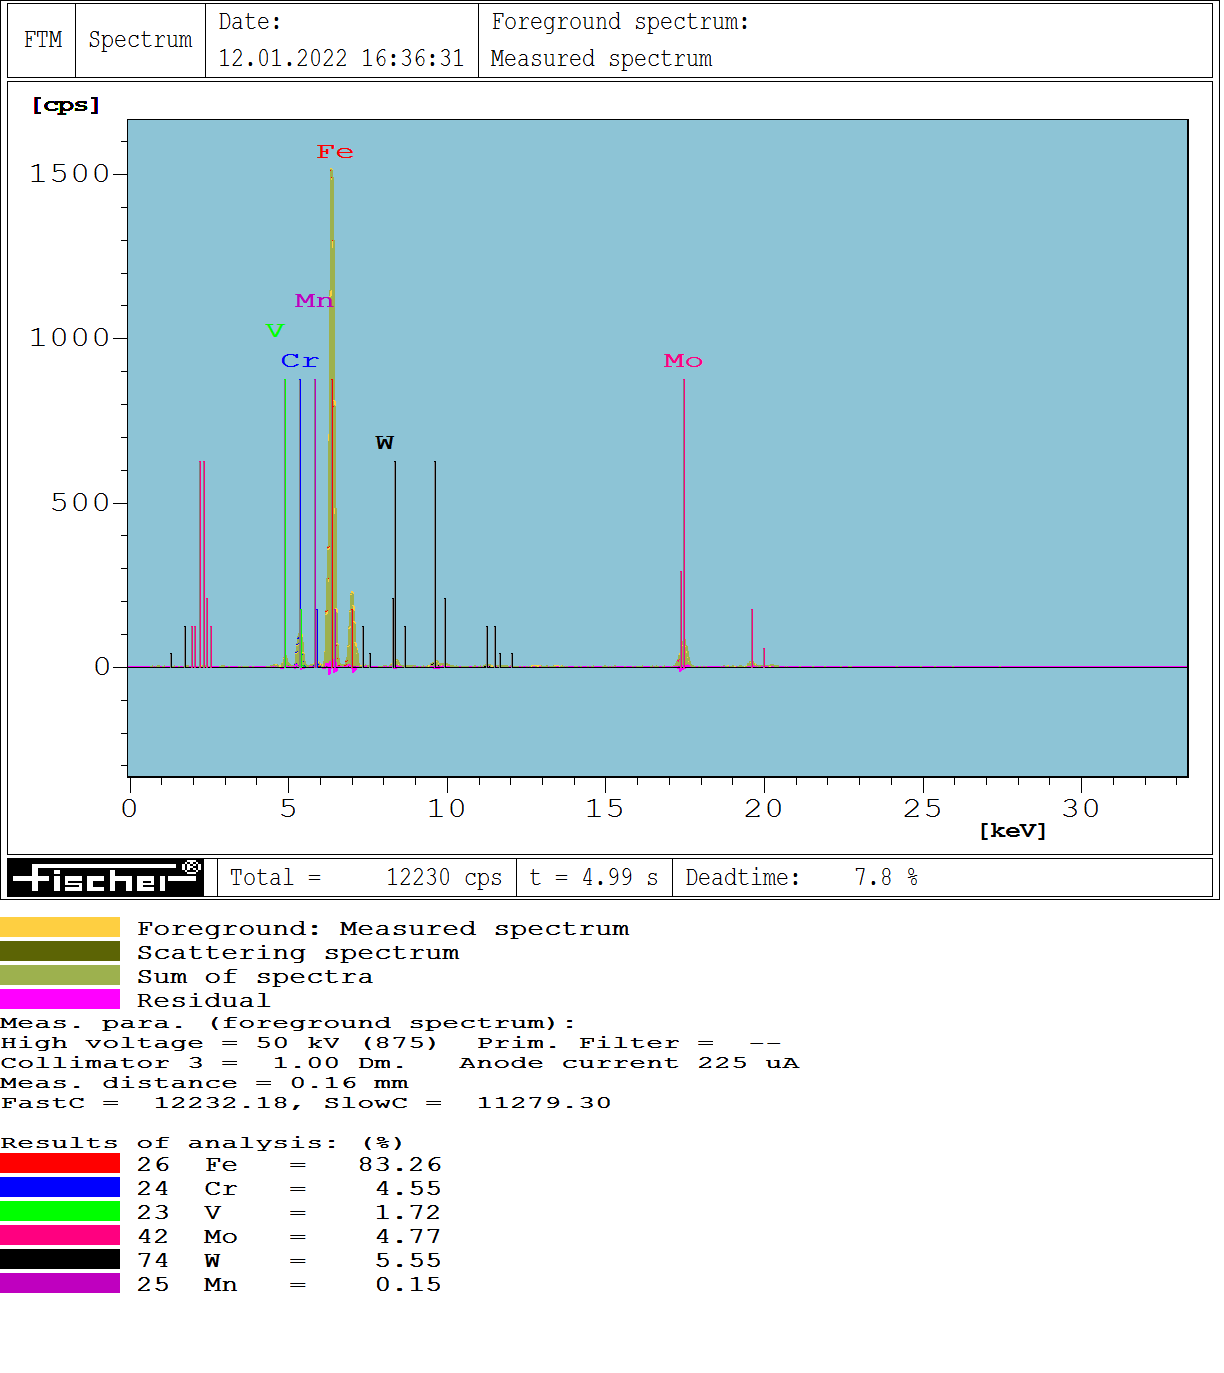
\includegraphics[width=0.5\textwidth]{3_Belichtungszeit_5s_3.png}
 \caption[Stahlprobe residual]{Residual Spektrum der Stahlprobe bei 50keV und ohne filter. Mit konzentration der Elemente}
 \label{fig:residual}
\end{figure}

Nicht alle vorhandenen Elemente wurden identifiziert. Co, S, P und Sn sind nur in einer sehr kleinen Konzentration in dem Stahl vorhanden so dass ihre Peaks sehr klein ausfallen und dadurch im Rauschen des Spektrums nicht identifiziert wurden. Die C K$\alpha_1 $ Peaks konnte im Spektrum nicht identifiziert da sie bei einer Energie von 0.227 keV liegt und damit eine zu niedrige Energie hat um sie mit dem zur Verfügung stehenden Messgerat zu Messen.\\

Die Si K$\alpha $ Peaks liegen bei 1.74 keV, welche in einem recht rausch starken Region des Spektrums liegt. In diesem Bereich sind auch die Al K$\alpha , \beta $ und die W M$\alpha_1 $ Peaks so das eine eindeutige Identifikation nicht möglich war. Es wurde dem entsprecht davon ausgegangen das die Si nicht Bestandteil der Probe ist und wurde deswegen nicht berücksichtigt.\\

Die Konzentrationsmessergebnisse sind mit den erwarteten Konzentrationen der Probe vergleichbar, durch die nicht erkannten Elemente sind jedoch recht große Ungenauigkeiten entstanden.\\

\begin{figure}[h]
 \centering
 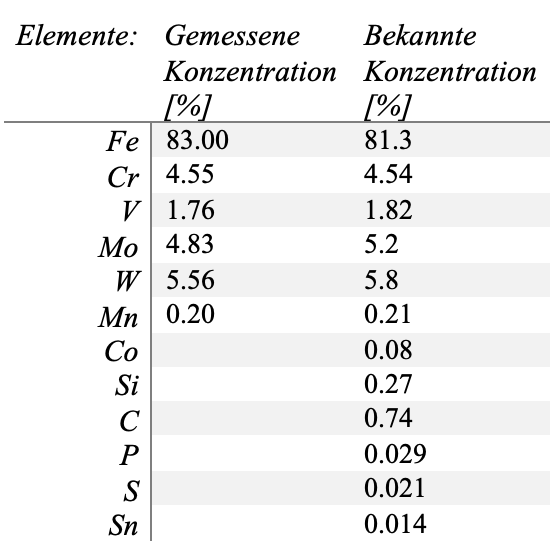
\includegraphics[width=0.5\textwidth]{Konzentration.png}
 \caption[Filter Tabelle]{Tabelle aller vorhandenen Elemente in der Stahlprobe.}
 \label{fig:Konzentration}
\end{figure}

Um die Reproduzierbarkeit zu überprüfen, wurden die Messungen mehrfach wiederholt zunächst wurden die Anregungsbedingenden verändert. Dafür wurden ein 500 µm Al Filter verwendet und die Höhe der Probe zum Detektor verändert. Anschließend wurden die Messungen ohne und mit dem 500 µm Al Filter an einer anderen Position der Probe wiederholt. Alle Messergebnisse sind auf der Tabelle \ref{fig:Stahl} im Appendix zu finden.\\
Es fällt auf das bei gleichbleibenden Anregungsbedingungen die Messergebnisse sehr ähnlich sind und damit auch reproduzierbar, dies wird auch durch eine kleine Standardabweichung bewiesen.
Bei Elementen mit einer sehr geringen Konzentration ändert sich die Ergebnisse zwischen unterschiedlichen Anregungsbedingungen verhältnismäßig viel, dies wird wieder mit der Standardabweichung aller gemessenen Konzentrationen aufgezeigt. Ein gutes Beispiel sind die Mn Peaks, beim Einsatz von Aluminiumfilter sind diese nicht mehr messbar. Das ist wahrscheinlich auf die geringe Konzentration von Mn in der Probe und die hohe Absorption von Aluminium in diesem Spektralbereich es Anregungsstahls zurückzuführen. Der Aluminium Filter sollte eigentlich helfen deinen höheren Kontrast zwischen rauschen/Streuung und den Fluoreszenzpeaks abzubilden, was hier nicht beobachtet wird. Durch eine längere Messzeit ist es wahrscheinlich möglich die Mn Konzentration wider zu messen. Um eine optimal Messzeit zu finden müssen weiter Versuche unternommen werden. \\
Nach Veränderung der Messposition auf der Probe ändern sich die Messergebnisse nicht maßgeblich, welches auf eine gute Homogenität der Probe deutet. Dabei liegt die Standard Abweichung immer auf einem sehr kleinen Wert bei der Messung unter gleichen Bedingungen und Positionen. Für Cr ist sie beispielsweise im Bereich von 0.02$\%$ für eine Konzentration von ca. 4,70$\%$.  Bei einer Veränderung der Position anderen sich die durchschnittlichen Konzentrationswerte nur gering. Beim Beispiel des Cr ist die Standard Abweichung der Durchschnittswerte bei 0,05$\%$ bei einem Durchschnittlichen Konzentration von 4,56$\%$. Selbs nach einem Positrons Wechsel konnten die Mn Peaks mit dem 500 µm Al Filter wie zuvor wieder nicht gemessen werden. \\



\subsection{Informationstiefe}

Durch die RFA Methode kann nicht das gesamte Volumen der Probe untersucht werden, da diese Methode relative oberflächensensitiv ist. Deswegen kann auch nicht garantiert werden, dass im Kern der Probe eine anderes Material vorhanden ist. Um solches Detail genauer zu untersuchen bieten sich andere Messmethoden an.
Um die Informationstiefe zu bestimmen wird sich Formel \ref{Eq:LAbs} und \ref{Eq:AbsKof} zunutze gemacht, dabei wird ein Anregungsstrahlphotonenenergie $E_0$ von 20,216keV angenommen die Austrittsphotonenenergie $E_I$ wir ebenfalls mit 20.216keV angenommen. Der Eintrittswinkel $\psi_1$ des Anregungsstrahls ist mit $90^\circ$  senkrecht zum Oberflache, während der Detektionswinkel $\psi_2$ bei $50^\circ$  liegt.

\begin{align}
\label{Eq:LAbs}
  L_{abs}=\displaystyle\frac{1}{\rho\cdot\mu*}
\end{align}

\begin{align}
\label{Eq:AbsKof}
  \mu* = \displaystyle\frac{\mu_i(E_0 = 20.216 keV)}{sin(\psi_1)} + \displaystyle\frac{\mu_i(E_i)}{sin(\psi_2)}
\end{align}

$E_0 =20.216 keV = E_0\\
\mu_i(E_0 = 20.216 keV) = mu_i(E_i)\\
\psi_1 = 90\circ\\
\psi_2 = 50\circ$\\

Um den Massenabsorptionskoeffizient $\mu_i$ zu ermitteln wird Gleichung \ref{Eq:MassAbsKof} verwendet hierbei werden Daten aus dem „X-RAY DATA BOOKLET“ genommen. 

\begin{align}
\label{Eq:MassAbsKof}
  \mu_i(E) = \displaystyle\frac{2\cdotr_e\cdot\lambda}{(A\cdotm_u}\cdotF^0_2
\end{align}

$\lambda (20.216 keV)= 0,0613 nm\\
r_e = 2.8179E-15 m\\
mu = 1.6605E-27 kg$\\

Da die Probe ein Stahllegierung ist, die aus mehreren Chemischen Elementen bestehet müssen die gleichen \ref{Eq:Sum} verwendet werden um die gesamte Dichte und Massenabsorptionskoeffizient zu erhalten.

\begin{align}
\label{Eq:Sum}
  \mu(E) = \sum\limits_{i=0}^{n} C\cdot\mu_i\\
  \rho = \sum\limits_{i=0}^{n} C\cdot\rho_i
\end{align}

Alle Verwendeten Absorptionskoeffizienten und Tabellarisch entnommen Werten sind in Tabelle \ref{fig:Intormationstiefe} zu finden zusammen mit den. 

\begin{figure}[h]
 \centering
 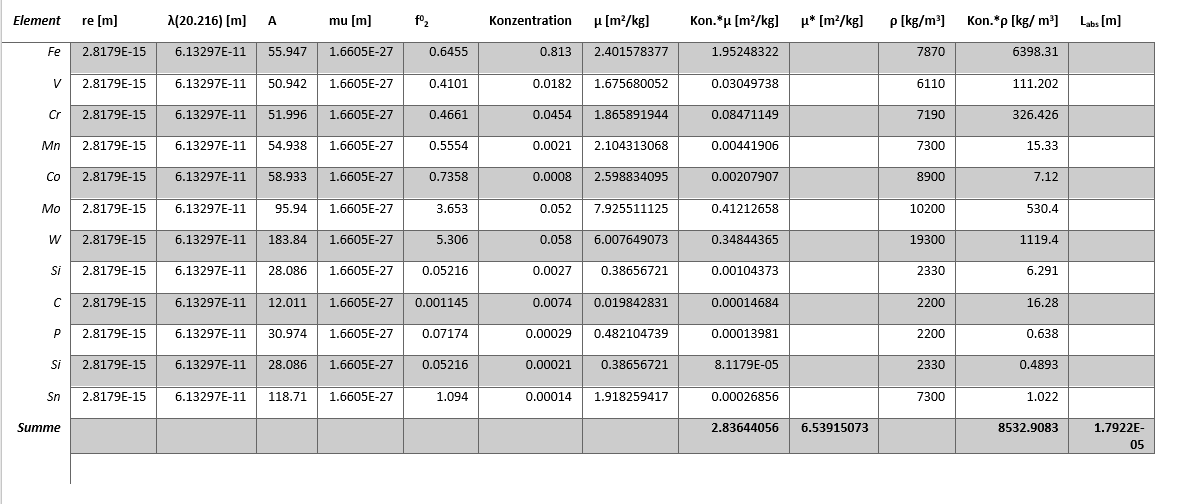
\includegraphics[width=1\textwidth]{Informationstiefe.png}
 \caption[Filter Tabelle]{Tabelle aller Verwendeten Koeffizienten, und errechnenden Teildichten und der Massenabsorptionskoeffizienten der Chemischen Elemente einer Stahllegierungsprobe.}
 \label{fig:Intormationstiefe}
\end{figure}

Die daraus resultierende Informationstiefe wird mit 17,9 $\mu m$ berechnet.

\subsection{C-Ni Mulilayer Spiegel}
Es wurde ein C-Ni Mulilayer Spiegel untersucht mit dem Ziel die Schichtdicken zu bestimmen und die optimale Wellenläge für eine Reflektion an diesem Spiegel zu ermitteln.\\

Mit Hilfe eines integrierten Software Tools des Messinstrumentes kann eine Schichtdicke gemessen werden, hierbei müssen einige bekannte Daten über die Probe in die Software eingetragen werden. Es muss das Chemische Element der zu messenden Schickt eingetragen werden, im Fall des C-Ni Mulilayer Spiegel wird nur die Ni Schichtdicke bestimmt, da die C Floreszenz Linie nicht im messbaren Bereich des Instrumentes liegt. Bei einer Messung wird die (kumulative) Gesamtschichtdicke aller Nickl Schichten zusammen gemessen, Im Fall des verwendeten C-Ni Mulilayer Spiegel betrug diese 15 Schichten. Die Schichtdicker einer einzelnen Schicht kann dann unter Annahme von uniform dicken Schichten errechnet werden. \\

Nach der Einrichtung der Anregungsbedingungen wurden jeweils 10 Messungen an 3 verschiedenen Positionen am Spiegel vorgenommen. Dabei wurde 50kV Hochspannung mit einem 500 µm Al Filter verwendet. Die mehrfachen Messungen wurden unternommen da die Messergebnisse zwischen einzelnen Messungen recht stark variiert, zudem muste die Homogenität der Schichtdicken über dem gesamten Spiegel sichergestellt werden.  Die Ergebnisse dieser Messungen sind in Tabelle \ref{fig:TabelleSpiegelMessung} zu finden, Die Durchschnittswerte an der jeweiligen Position zusammen mit der zugehörigen Standardabweichung wird dort ebenfalls aufgeführt. 

\begin{figure}[h]
 \centering
 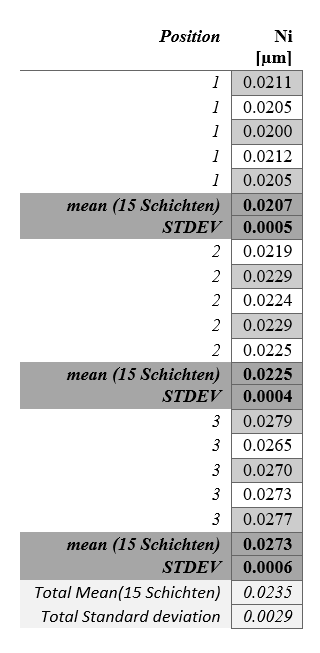
\includegraphics[width=0.25\textwidth]{SpiegelMessung.png}
 \caption[Tabelle C-Ni Spiegel]{Tabelle der Ni Sichtdicke Messungen}
 \label{fig:TabelleSpiegelMessung}
\end{figure}

Da die Schicktdickenverhältnisse zwischen der C und der Ni Schicht mit $\displaystyle\frac{dC}{dNi} = \displaystyle\frac{55}{45}$ bekannt ist, kann damit auch die Schichtdick der C Schickt erreichten werden. Unter zur Hilfename von der Gleichung \ref{Eq:Periodenlänge} kann die Periodenlänge d bestimmt werde.

\begin{align}
\label{Eq:Periodenlänge}
  d = dC + dNi =  \displaystyle\frac{55}{45}*dNi+dNi = \displaystyle\frac{20}{9}
\end{align}

Die Durchschnittliche kumulative Gesamtdicke des Nickels wurde mit 23,5 nm gemessen. Damit wurde berichtet das eine Ni Schicht 1,56 nm beträgt. Unter Zuhilfenahme von Gleichung \ref{Eq:Periodenlänge} wurde Eine Periodenlänge d von 3,47 nm berechnet.\\
Durch die nutzung der Bragg Bedingung \ref{Eq:Bragg} kann nun die bestmögliche Photonenenergie für eine Reflektion an diesem Spiegel bestimmt. \\

\begin{align}
\label{Eq:Bragg}
    m\delta = 2 d sin(\theta)
\end{align}

Dabei wurden die beiden Einfallswinkel $\theta$ von 90° und 45° Verwendet, zusammen mit Reflektionsordnung von m=1.  Bei einem Einfallswinkel von 90° ist die optimale Energie 178,5 eV ($\lambda$ = 6,95 nm), und bei einem Einfallswinkel von 45° ist sie 252,5 eV ($\lambda$ = 4,91 nm). Die Ergebnisse sind in Tabelle \ref{fig:TabelleSpiegelErgebisse} aufgeführt. Es sind auch Energien gut geeigneten an diesem Spiegel mit demselben Einfallswinkel zu reflektieren, wenn eine höhere Reflectionsordnung gewählt wird.\\
\begin{figure}[h]
 \centering
 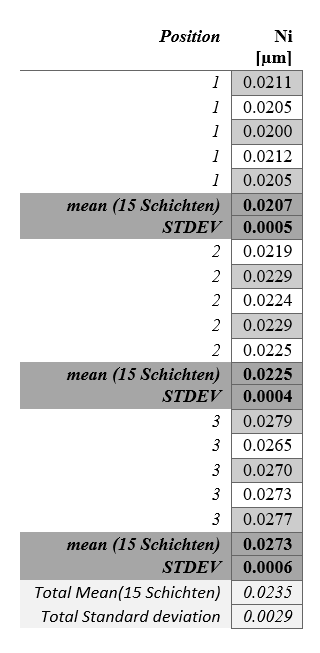
\includegraphics[width=0.25\textwidth]{SpiegelMessung.png}
 \caption[Tabelle C-Ni Spiegel]{Tabelle das C-Ni Multilayer Spiegel, Ergebnisse der Schichtdicke von einer Ni und C Schicht, der  Periodenlänge und der Optimale Photonenenergie bei einer 90° und 45° Reflektion}
 \label{fig:TabelleSpiegelErgebisse}
\end{figure}


\begin{figure}[h]
 \centering
 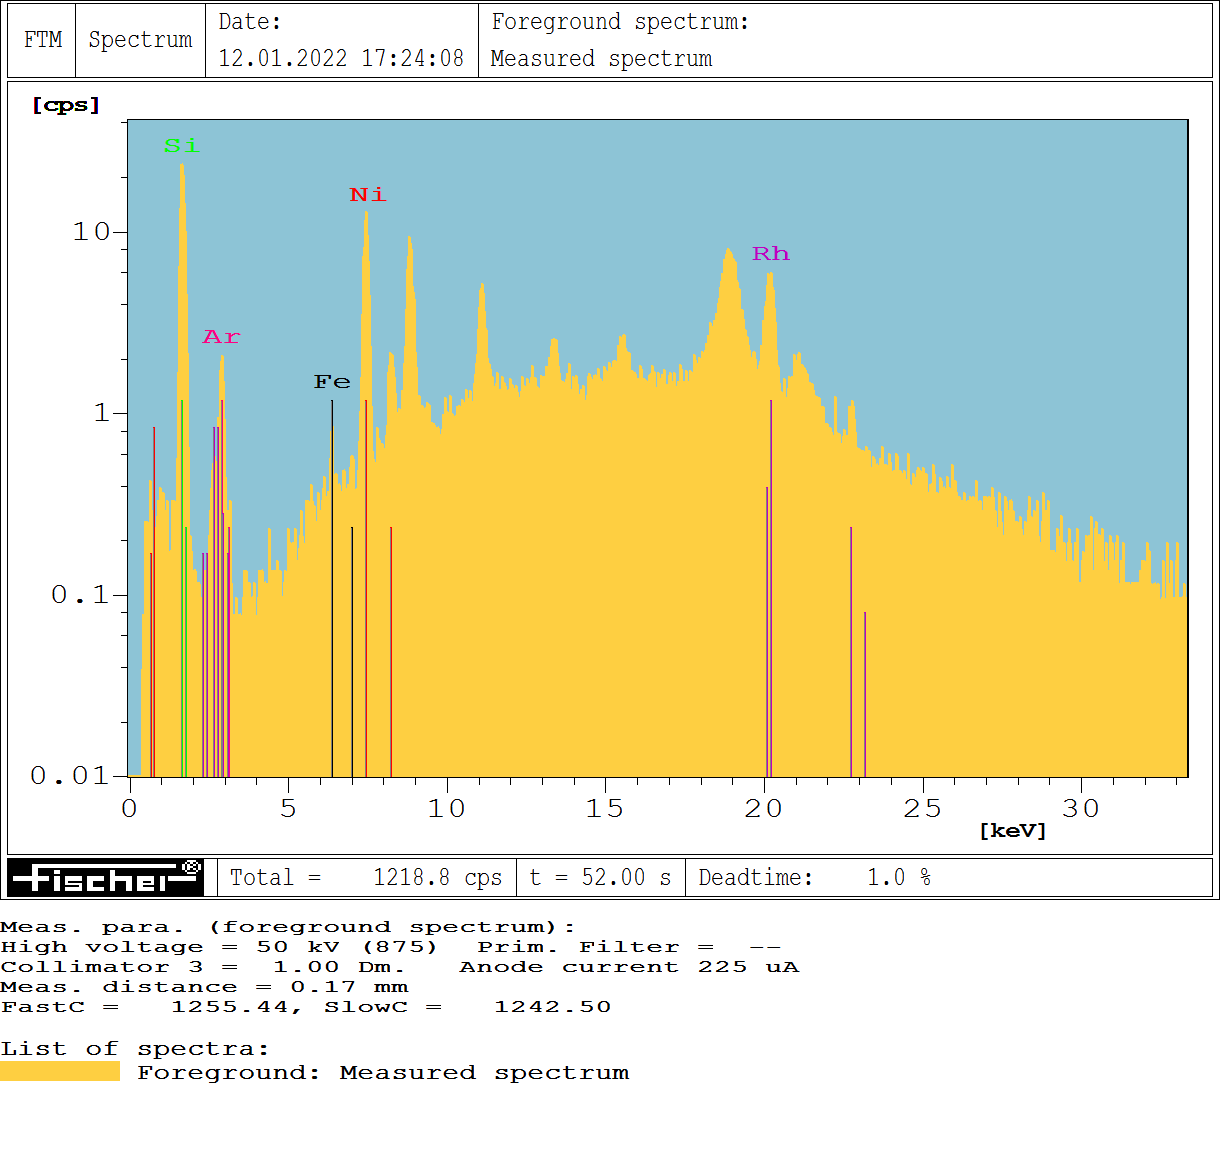
\includegraphics[width=0.5\textwidth]{2_Spektrum2.png}
 \caption[C-Ni Spiegel]{Spektrum des C-Ni Spiegel auf Si Substrat, Schichtdickenverhäldtis 55:45, Gesamtschichtdicke 52.2$\pm$6 nm }
 \label{fig:C-Ni Spiegel}
\end{figure}


\subsection{Wasserprobe}
In diesem Teil wurde eine Trinkwasserprobe der Technische Universität Berlin untersucht, um festzustellen ob irgendwelche Kontaminationen im Trinkwasser vorhanden sind. Die Wasserprobe selbst weist keine Hinweise auf Verunreinigungen oder Kontamination des Wassers auf, es wurden lediglich die folgenden Elemente identifiziert: P, Ar, Ca, Fe, Ni, Cu & Zn.\\
Jedoch muss nach der Betrachtung der Referenzmessung der Plastikkappe in dem die Wasserprobe aufbewahrt wird, die meisten der gemessenen Elemente auf eine Verneigung durch die Plastikkappe zurückgeführt betrachtet werden. Hier wurden widere die Elemente, Ar, Ca, Fe, Ni, Cu & Zn und zusätzlich ein Ar Peaks Gemessen. Zudem ist die Intensität der Fe, Ni & Zn Peaks sehr viel stärker ausgeprägt als in der reinen Wasserprobe.\\
Der genaue Ursprung dieser stark ausgeprägten Peaks ist nicht einfach zu erklären, da die Plastik kappe aus einem Kunststoff besteht, wahrscheinlich PET, in welchem diese Elemente nicht verwendet werden. Der Grund für das Vorhandensein dieser könnet durch eine Kontaminierung der Kappe zu Grunde liegen, es könnten zum Beispiel Nickelpulver in dem Behälter der Kappe gelagert worden sein. Diese Verunreinigung ist möglicherweise in den porösen Kunststoff eingedrungen welcher nun gemessen wurde. Eine andere Möglichkeit könnte auch die Verunreinigung der Plastikkappe durch einen Verschmutztem Lappen nach dem Spülen im Wasser sein. Um diesen Peaks genau auf den Grund zu gehen müssen weiter Untersuchungen durchgeführt werden, eine Verunreinigung erscheint anhand der Vielzahl der als Pulvers anwesenden Proben in diesem Labor jedoch am wahrscheinlichsten. Das vorhanden sein des Arsens ist zwar fragwürdig aber nicht völlig undenkbar, da Arsen manchmal in Legierungen zu finden ist. Ein Beispiel dafür ist Weißkupfer welchen für versilberungen genutzt wurde. Auch hier ist die Verneigung wahrscheinlich durch Pulver im Behalte oder Lappen am wahrscheinlichsten.\\
Trotz dem stark kontaminierten Probenhalter sind einige Rückschlüsse über das Wasser möglich. Es sind zwar die gemessenen Peaks Ca, Fe, Ni, Cu & Zn erklärbar da sie normale Bestandteile des Trinkwassers sind, ihre qualitative und quantitative Bestimmung ist jetzt allerdings nicht mehr möglich. Das Fehlen der Arsen Peaks in der Wasserprobe ist wahrscheinlich durch eine geringe Konzentration oder Rachen im Spektrum zu erklären. Dass einzige identifizierte Element welchen ausschließlich im Wasser gemessen wurde ich Phosphor. Phosphor lässt sich durch eine Zugabe im Trinkwassers von Phosphaten erklären, welche zum Korrosionsschutz der Leitungen dient soll und ist damit auch ein normaler Bestandteil von Berliner Trinkwasser ist.\\
Schwermetalle wie Blei konnten nicht festgestellt werden, ebenso wie andere Verunreinigungen die manchmal beobachtet werden. Das deutet auf ein kontaminationsfreies Trinkwasser hin. Um dies jedoch zweifelsfrei zu bestimmen müssen die Messungen widerholt werden. Dabei ist auf einen kontaminationsfreien Probenhalter zu achten. Zuzüglich ist eine längere Mußezeit wahrscheinlich von Vorteil um das Rauschen weiter zu minimieren.



\begin{figure}%
    \centering
    \subfloat[\centering Wasserprobe ]{{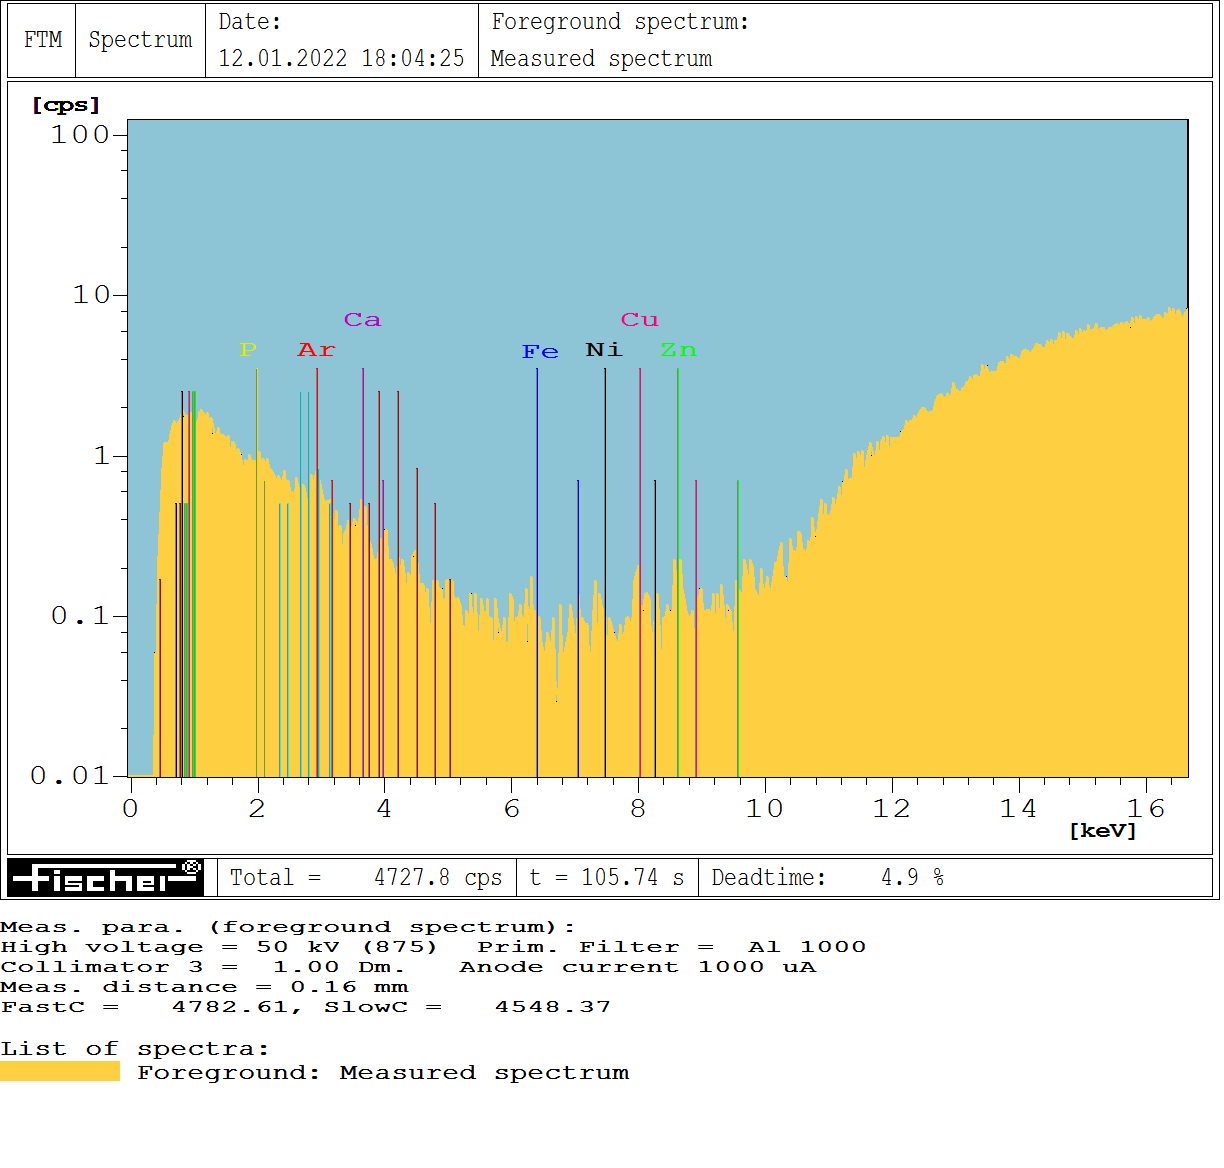
\includegraphics[width=7cm]{2_Wasserprobe_2.png} }}%
    \qquad
    \subfloat[\centering Plastik Kappe ]{{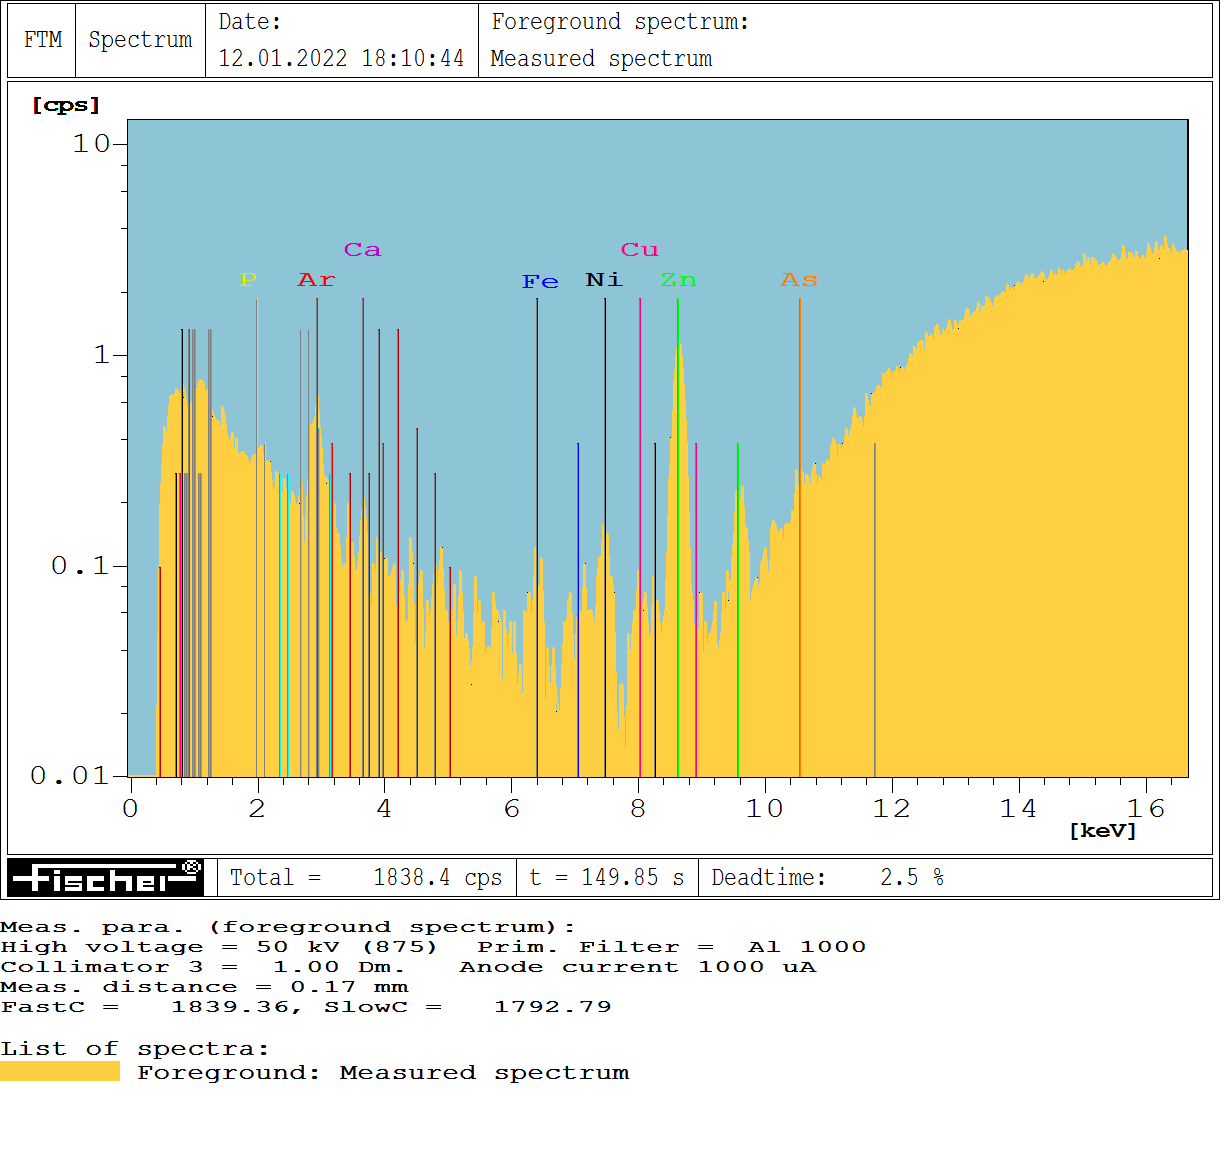
\includegraphics[width=7cm]{3_Wasserprobe_3.png} }}%
    \caption{Spektrum einer Wasserprobe und Referenz Spektrum des Behälter (Plastik Kappe)}%
    \label{fig:example}%
\end{figure}
